
\section{Introduction}
\label{sec:introduction}

Stellar bow shocks are produced by the relative motion between a star
and its surrounding medium, and are commonly detected as curved arcs
of emission at optical \citep{Gull:1979a, Brown:2005a}, infrared
\citep{van-Buren:1988a, Kobulnicky:2016a}, or radio
\citep{van-Buren:1990a, Benaglia:2010a} wavelengths.  The canonical
theory for these objects is that they are formed by a two-shock
interaction between the stellar wind and the interstellar medium
\citep{Pikelner:1968a, Dyson:1972a}, which is distorted due to the
supersonic motion of the star \citep{Baranov:1970a, Wilkin:1996a}.  In
some instances, however, the absorbed stellar radiation pressure may
be more important than the stellar wind in providing the inner support
for the bow shell \citep[Paper~I]{Henney:2019a} and this may even be
sufficient to break the collisional coupling between gas and dust
grains \citep[Paper~II]{Henney:2019b}.  We have proposed a diagnostic
method to distinguish between these cases, based on the bow shock size
and the luminosity ratio between the bow shock and the star
\citep[Paper~III]{Henney:2019c}. In other cases, the appearance of an
infrared emission arc may be due to the illumination of the inner wall
of an asymmetrical cavity \citep{Mackey:2016a}, rather than the
formation of a dense shell, in which case the relative velocity of the
star may be subsonic with respect to its surroundings
\citep{Mackey:2015a}.

The largest number of bow shocks have been detected around high-mass
OB stars, via their mid-infrared dust emission \citep{van-Buren:1995a,
  Noriega-Crespo:1997b, Povich:2008a, Kobulnicky:2010a, Peri:2012a,
  Peri:2015a, Sexton:2015b, Kobulnicky:2016a, Bodensteiner:2018a}, and
these have typical sizes ranging from \SIrange{0.01}{1}{pc}. In
particularly dense environments, such as the inner Orion Nebula
\citep{Smith:2005a} and the Galactic center region
\citep{Geballe:2004a} they may be as small as \SI{0.003}{pc} and emit
at near-infrared wavelengths \citep{Tanner:2005a,
  Sanchez-Bermudez:2014a}.  Cometary ultracompact \hii{} regions
detected at radio wavelengths \citep{Reid:1985a, Wood:1989a,
  Klaassen:2018a} have also been interpreted as bow shocks
\citep{van-Buren:1990a, Mac-Low:1991a}, although alternative models,
such as a champagne flow caused by steep density gradients
\citep{Cyganowski:2003a, Arthur:2006a, Immer:2014a, Steggles:2017a},
are favored in many cases.  This illustrates a broader point: that it
can be difficult to identify bow shocks from morphology alone, since
other processes can give rise to emission arcs.  In particular, curved
ionization fronts, as seen in evaporating globules \citep{Sahai:2012b}
and proplyds \citep{ODell:1993a} can be mistaken for bow shocks.
Kinematic observations can potentially resolve such ambiguities but
are not always available.

Stellar bow shocks are also observed around other types of stars. Bow
shocks around cool red supergiant and asymptotic giant branch stars
are detected at mid-infrared and far-infrared wavelengths
\citep{Ueta:2006a, Ueta:2008a, Sahai:2010a, Cox:2012a}.  Pulsar bow
shock nebulae are detected principally by their H\(\alpha\) emission
\citep{Kulkarni:1988a, Brownsberger:2014a}.  In the Orion Nebula (M42,
NGC~1976), at least three different classes of stellar bow shock have
been identified. As well as a small number of OB bow shocks
\citep{Smith:2005a, ODell:2001c}, bow shocks are also seen around the
closest proplyds to the dominant O~star \thC{} \citep{Hayward:1994a,
  Bally:1998a, Robberto:2005a}.  The proplyds \citep{ODell:2008b} are
photoevaporating protoplanetary disks around low-mass young stars
\citep{Johnstone:1998a} and the bow shocks have been modeled as the
interaction between the disk's ionized photoevaporation flow and the
supersonic stellar wind from \thC{} \citep{Garcia-Arredondo:2001a}.
The third class of Orion Nebula bow shock is the LL~Ori-type objects
\citetext{\citealp{Gull:1979a}; \S~5 of \citealp{Bally:2000a}; \S~3.2
  of \citealp{Bally:2001a}; \citealp{Henney:2013a}}, which tend to be
found in the outer regions of the nebula.  These are probably due to
interactions between the Orion Nebula's champagne flow
\citep{Zuckerman:1973a} and outflows from T~Tauri stars, which may or
may not be proplyds \citep{Bally:2000a, Gutierrez-Soto:2015a}.

\begin{figure}
  \centering
  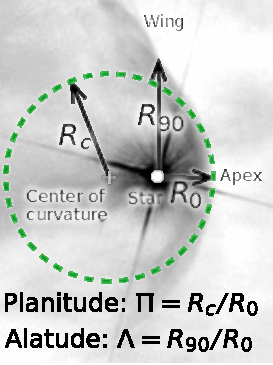
\includegraphics[width=0.6\linewidth]{figs/obs-shape-terminology}
  \caption[Terminology]{Terminology employed in this paper to describe
    bow shock shapes, following \citet[Paper~0]{Tarango-Yong:2018a}.}
  \label{fig:obs-shape-terminology}
\end{figure}

The shapes of stellar bow shocks are frequently compared with what has
become known as the \textit{wilkinoid} surface \citep{Cox:2012a},
which is the result of the idealized interaction between a spherical
wind and a plane-parallel stream in the hydrodynamic thin-shell
approximation.  Numerical approximations to this shape were used by
various authors \citep{Baranov:1971a, Mac-Low:1991a} before an elegant
analytic solution was found by \citet{Wilkin:1996a} and extended to
the case of interaction between two spherical winds
\citep{Canto:1996}.  In \citet[hereafter, Paper~0]{Tarango-Yong:2018a}
the study of bow shock shapes and their projection on the plane of the
sky was formalized. The term \textit{cantoid} was introduced for the
\citet{Canto:1996} family of shapes, together with \textit{ancantoid}
for a generalization to the case where one of the winds is
anisotropic, as is appropriate for the proplyds.  In addition, Paper~0
proposed the use of two dimensionless parameters, \textit{planitude}
and \textit{alatude}, to describe a general bow shock shape, which we
illustrate in Figure~\ref{fig:obs-shape-terminology}.  The planitude,
\(\Pi = R_c / R_0\), measures the flatness of the bow shock apex, where
\(R_0\) is the star--apex distance and \(R_c\) is the radius of
curvature measured at the apex.  The alatude,
\(\Lambda = R_{90}/R_0\), measures the openness of the bow shock wings,
where \(R_{90}\) is the lateral size of the bow, measured from the
star in the direction perpendicular to the star--apex direction.

In this paper, we investigate the shapes of stellar bow shocks by
calculating the distributions of planitude and alatude for different
classes of bow shock source.  The remainder of the paper is organized
as follows. In \S~\ref{sec:mid-infrared-arcs} we present an analysis
of the shapes of several hundred bow shock candidates associated with
OB stars from the \SI{24}{\um} survey of \citet{Kobulnicky:2016a}.
Our algorithm for automatically fitting and tracing the shapes is
described in \S~\ref{sec:autom-trac-fitt}, together with our ``star
rating'' system for evaluating the fit quality, while in
\S~\ref{sec:ob-shapes} we locate the sources on the planitude--alatude
plane.  In \S~\ref{sec:corr-size} we study the correlations amongst
non-shape parameters of the bow shock sources, such as angular size
and stellar magnitude, while in \S~\ref{sec:corr-shape} we explore the
correlations between these parameters and the planitude and alatude.  In
\S~\ref{sec:far-infrared-arcs} we compare with results for bow shocks
around cool luminous stars and in \S~\ref{sec:stat-emiss-line} we
compare with results for stationary emission-line arcs in the Orion
Nebula.  In \S~\ref{sec:discussion} we discuss the implications of our
findings for physical models of bow shock formation in the different
classes of sources, and in \S~\ref{sec:conclusion} we summarise our
results.  Further details of the statistical tests that we have
applied are provided in Appendix~\ref{sec:distr-p-values} and a simple
model for time-dependent oscillations of the bow shock surface is
presented in Appendix~\ref{sec:perturbed-bows}.

% Bowshocks from red supergiants \citep{Meyer:2014a}.  Simluations of AGB bows \citep{Villaver:2012a}, RSG \citep{Mohamed:2012a}


% Wolf Rayet stars give bigger bow shocks (e.g., WR~128 \citealp{Moffat:1998})

% Interaction of wind with photoevaporation flow \citep{Dyson:1975a}

% HMXRB in external galaxies, possible bowshock in LMC~X-1 \citep{Hyde:2017a}.

% Wolf-Rayet bow shock nebulae \citep{Dyson:1989a}

% Non-thermal radio emission from BD+43~3654 \citep{Benaglia:2010a}, has
% been searched for but

% Supersonic pulsar wind nebulae \citep{Kargaltsev:2017a}


%%% Local Variables:
%%% mode: latex
%%% TeX-master: "obs-bowshocks"
%%% End:
